\documentclass[crop,tikz]{standalone}
\usetikzlibrary{shapes,decorations,arrows,calc}
\usetikzlibrary{decorations.pathmorphing}
\begin{document}

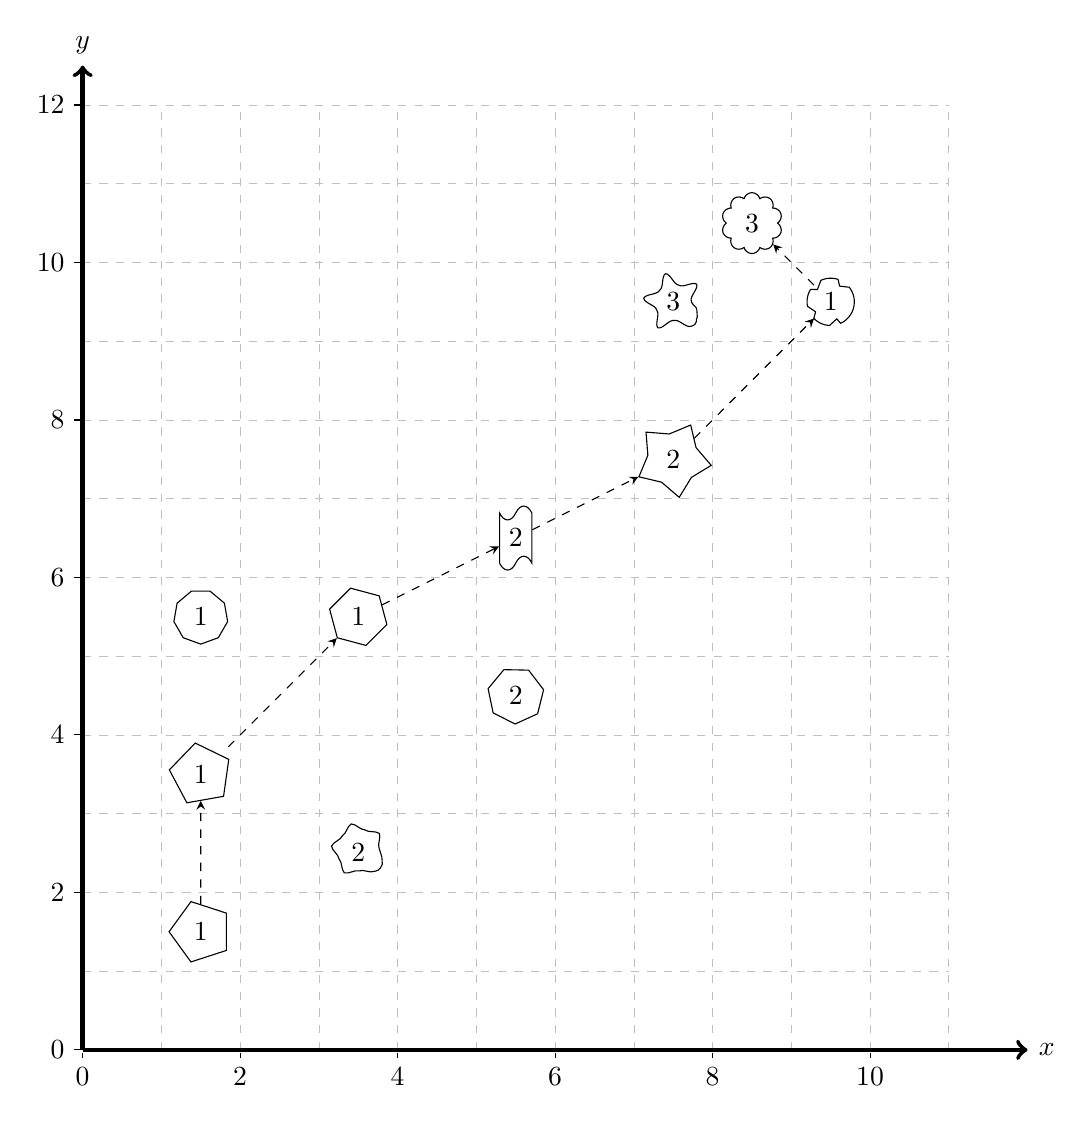
\begin{tikzpicture}
\draw[
	help lines, 
	color=gray!50,
	dashed,
	shift={($(0, 0) - (0.5, 0.5)$)},
] (0,0) grid (11,12);
\draw[->,ultra thick] (-0.5,-0.5)--(11.5,-0.5) node[right]{$x$};
\draw[->,ultra thick] (-0.5,-0.5)--(-0.5,12) node[above]{$y$};

\foreach \x in {0,2,4,6,8,10}
    \draw ({\x cm-0.5 cm},{-0.5cm - 1pt}) -- ({\x cm-0.5cm},{-0.5cm -3pt})
        node[anchor=north] {$\x$};
\foreach \y in {0,2,4,6,8,10,12}
    \draw ({-0.5cm - 1pt},{\y cm - 0.5cm}) -- ({-0.5cm - 3pt},{\y cm - 0.5 cm}) node[anchor=east] {$\y$};

\node (0) at (1,0) {};
\node[draw,regular polygon,regular polygon sides=5, shape border rotate=10] (1) at (1,3) {1}; 
\node[draw,regular polygon,regular polygon sides=5, shape border rotate=90] (-1) at (1,1) {1}; 
\node (2) at (3,2) {2}; 
\node[draw,regular polygon,regular polygon sides=9, shape border rotate=20] (3) at (1,5) {1}; 
\node[draw,regular polygon,regular polygon sides=6, shape border rotate=45] (4) at (3,5) {1}; 
\node[draw,regular polygon,regular polygon sides=7, shape border rotate=76] (5) at (5,4) {2}; 
\node[draw,tape] (6) at (5,6) {2}; 
\node[draw,star,star points=5, shape border rotate=45] (7) at (7,7) {2}; 
\node (8) at (7,9) {3}; 
\node (9) at (9,9) {1}; 
\node[draw,cloud] (10) at (8,10) {3}; 

\draw[decorate,decoration={straight zigzag,meta-segment length=0.2cm}] (9,9) circle (0.3);
\draw[decorate,decoration={snake,amplitude=1pt}] (3,1.95) circle (0.3);
\draw[decorate,decoration= {snake,amplitude=2pt}] (7,8.9) circle (0.3);

% \draw[dashed,->,>=stealth] (0) edge node[auto] {2} (2);
% \draw[dashed,->,>=stealth] (2) edge node[auto] {3} (4);
% \draw[dashed,->,>=stealth] (4) edge node[auto] {2.23\ldots} (6);
% \draw[dashed,->,>=stealth] (6) edge node[auto] {2.23\ldots} (7);
% \draw[dashed,->,>=stealth] (7) edge node[auto] {2.82\ldots} (9);
% \draw[dashed,->,>=stealth] (9) edge node[auto] {1.41\ldots} (10);
% \draw[dashed,->,>=stealth] (0) edge (-1);
\draw[dashed,->,>=stealth] (-1) edge (1);
\draw[dashed,->,>=stealth,shorten <=4pt] (1) edge (4);
\draw[dashed,->,>=stealth] (4) edge (6);
\draw[dashed,->,>=stealth] (6) edge (7);
\draw[dashed,->,>=stealth] (7) edge (9);
\draw[dashed,->,>=stealth] (9) edge (10);

\end{tikzpicture}

\end{document}
